\documentclass[../main.tex]{subfiles}
\graphicspath{{\subfix{../IMAGES/}}}

\begin{document}
\localtableofcontents

\subsection{What is an energy system}
General conversion factors for energy : \\
\begin{table}[hbt!]
    \centering
    \begin{tabular}{|c|c|c|c|c|c|}
        \hline
        From $\backslash$ To & TJ & Gcal & Mtoe & MBtu & GWh \\\hline
        TJ & 1 & 238.8 & $2.388 \cdot 10^{-5}$ & 947.8 & 0.2778\\ \hline
        Gcal & $4.1868 \cdot 10^{-3}$ & 1 & $10^{-7}$ & 3.968 & $1.163 \cdot 10^{-3}$\\ \hline
        Mtoe & $4.1868\cdot 10^{4}$ & $10^7$ & 1 & $3.968 \cdot 10^7$ & 11630\\ \hline
        MBtu & $1.0551 \cdot 10^{-3}$ & 0.252 & $2.52 \cdot 10^{-8}$ & 1 & $2.931 \cdot 10^{-4}$\\ \hline
        GWh & 3.6 & 860 & $8.6 \cdot 10^{-5}$ & 3412 & 1\\ \hline
    \end{tabular}
\end{table}

The energy system comprises all components related to the production, conversion, delivery and use of energy : 
\begin{itemize}
    \item Demand : \begin{itemize}
        \item Energy service : why we use energy\\
        \item Useful energy : the energy form at the very end\\
    \end{itemize}
    \item Conversion \& transmission : \begin{itemize}
        \item Final energy\\
        \item Distribution : how it comes to your place\\
        \item Secondary energy : what is available before you transport it\\
        \item Conversion : how it becomes something usable\\
    \end{itemize}
    \item Resource : Primary energy (what was harvested at the beginning)\\
\end{itemize}

To describe it, we can use a \textbf{Sankey diagram}. With on the left the resources, then the conversion technologies and then the demands. Electricity is about $25\%$ of the final energy use. \\

\subsubsection{Demands}
How can we reduce the demands? \begin{itemize}
    \item Energy sobriety : avoid excess and waste\\
    \item Energy efficiency at end-use level : ensure same service but with less demand\\
    \item Energy efficiency at conversion level : ensure same end-use supply but improve the use of resources\\
\end{itemize}

\subsubsection{Conversion}
It is necessary to compare different options to convert energy in the form we need. 
For example, a house could be heated using different way : natural gas and a boiler which has an efficiency of about $90\%$ but which needs to be refined first; wood alongside a boiler which would only have the efficiency of the boiler; natural gas converted to electricity with an electric heater (about $95\%$ efficiency); or solar panel alongside a heat pump which has an efficiency of $400\%$.\\

A lot of energy may be lost when : \begin{itemize}
    \item converting secondary into end-use energy\\
    \item producing secondary energy\\
\end{itemize}

\subsection{Status and challenges}
\begin{itemize}
    \item Unconventional : not economic or not feasibly recoverable
    \item Ressources : detected, cannot yet be recovered profitably
    \item Reserves : can be recovered
\end{itemize}
There still is enough reserve of oil to last $50$ years and of coal to last $100$ years. \\

\quad \underline{Non-conventional oil resources :}\\
They lead to more difficult operating conditions and greater environmental/economic risks. Currently not economically interesting to extract.\\

The higher the price of oil, the more competitive renewable resources are as well as non-conventional resources.\\

\subsubsection{The material challenge}
\begin{itemize}
    \item Rare earths : (17 elements) : not necessarily rarem supply risk, increasing risk
    \item Rare metal : low abundance metals
    \item Critical materials : strategic sourcing
\end{itemize}


The chain is less diversified : China is a key player for rare earths.\\

\subsubsection{The cost challenge}
Costs of low-carbon technologies (LCOE). These costs depend on the installed capacity and the type of energy. In 2020, renewables were competitive in Europe but not in Japan.\\

\subsubsection{The energy and power density challenge}

Renewables require large areas : \begin{itemize}
    \item Bioethanol : $\simeq 0.05,0.15 W/m^2$
    \item Wind : $\simeq 2,10 W/m^2$
    \item Hydro : $\simeq 10,15 W/m^2$
    \item Solar : $\simeq 5,20 W/m^2$
\end{itemize}
The average power use of a Swiss citizen is $3.2kW/p$.

\subsubsection{The efficiency challenge}
\quad \underline{First principle :}\\
Energy is conserved, neither created nor destroyed.\\

Energy for heat and mechanical engines : \begin{itemize}
    \item nuclear : $\eta_I = \frac{W^-}{Q^+} = \frac{\text{Power output}}{\text{Nuclear fuel energy}} \simeq 30-35\%$
    \item wind : $\eta_I = \frac{W^-}{W^+} = \frac{\text{Power output}}{\text{Wind kinetic energy}} \simeq 20-40 \%$
    \item coal : $\eta_I = \frac{W^-}{Q^+} = \frac{\text{Power output}}{\text{Coal chemical energy}} \simeq 35-40\%$
    \item heater : $\eta_I = \frac{Q^-}{W^+} = \frac{\text{Heat output}}{\text{Electricity input}}$
    \item solar collector : $\eta_I = \frac{Q^-}{Q^+} = \frac{\text{Heat output output}}{\text{Solar radiation}} \simeq 70-80\%$
\end{itemize}

\subsubsection{Second principle}
Can we produce as much work as we get heat?\\

Impossible to get as much power out as heat in from a given power plant. Because of entropy generation, $100\%$ is not achievable.\\

Carnot efficiency (maximum theoretical efficiency): \begin{equation}
    \theta = 1-\frac{T_0}{T_Q}
\end{equation}
With $T_0$ the ambient temperature and $T_Q$ the heat transfer temperature. \\
Not all heat can be converted into electricity but all electricity can be converted into head. 

\quad \underline{Exergy :}\\
The useful work potential (how much electrical/mechanical work can be produced from a given energy source).\\
\begin{itemize}
    \item For mechanical/electrical flows : exergy = energy = W
    \item For fuels : exergy $\simeq$ higher heating value (HHV)
    \item For heat : exergy = enery x Carnot factor $= Q \theta$
\end{itemize}

The second law of efficiency is given by : \begin{equation}
    \eta_{II} = \frac{\text{what you get}}{\text{what you would get in the ideal case}} = \frac{W^-}{Q^+ \theta}
\end{equation}

\subsubsection{Economic evaluation}
The capital costs are associated with the capital to build a new plant, assessed over the plant lifetime. The O \& M costs are related to the fuel, labour, electricity, maintenance costs and operating time, evaluated over a year. \\

The equipment cost can be computed from : \begin{equation}
    C_{pc,i} = C_{pc,i, ref} (\frac{S_{pc,i}}{S_{pc,i,ref}})^\alpha
\end{equation}
Where \begin{itemize}
    \item $C_{pc,i,ref}$ the equipment cost at the reference size
    \item $S_{pc,ref}$ the reference size expressed in $kg/s$, $MW$, $m^3$
    \item $S_{pc}$ the equipment size that we evaluate
    \item $\alpha$ the cost coefficient which takes into account the economics of scale (usually 0.6)
\end{itemize}

If the price information comes from correlations in the past, we may need to take into account inflation over time : $C_{pc,i} = C_{pc, i, t_0} (\frac{I_2}{I_1})$.\\

The total cost is then : \begin{equation}
    C_{inv, tot} = f_{inst} \sum_i C_{pc,i} [USD]
\end{equation}
With $C_{inv}$ the total capital cost, $f_{inst}$ the installation factor (usually 4).\\

The annualised capital cost is then : \begin{equation}
    C_{inv} = \frac{i(1+i)^n}{(1+i)^n-1} C_{inv,tot} [USD/year]
\end{equation}
Where $C_{inv}$ the annualised capital cost in USD/year, $C_{inv,tot}$ the total capital cost over the plant lifetime, $i$ the interest rate and n the plant lifetime.\\

The annual capacity factor $c_p = \frac{t_{op}}{8760}$.\\
The maintenance cost $C_{om} = C_{fuel} + C_{maint} + C_{mp} [USD/year]$ with $C_{fuel} = \dot{m}_{fuel} c_{fuel} t_{op}$, $C_{maint} = f_{maint} C_{inv,tot}$ where $f_{maint} \simeq 1-10\%$.\\

The capacity factor measures how many hours in a given period the power plant operates at full capacity.\\

The levelised cost of energy (LCOE) can be defined as the present value of the price of the produced form of energy. It allows for a direct comparison of the costs of electricity generation projects.\\
\begin{equation}
    LCOE = \frac{(\frac{i(1+i)^n}{(1+i)^n-1})C_{inv,tot} + C_{om}}{W_{tot}} [USD/Wh]
\end{equation}
Where $C_{inv}$ the total capital cost of electricity generation plant expressed in USD, $C_{om}$ the total O \& M cost over a year, $i$ is the discount rate of the plant, n the plant lifetime and $W_{tot} [Wh/year]$ the total electricity production over a year.\\


Technological advances that improve performance of a given technology or its production efficiency will result in lowed production cost. This can be defined by : $c_{inv, i, t2} = c_{inv, i, t1} (\frac{S_{i,t2}}{S_{i,t1}})^\beta$ where $c_{inv,i,t2}$ is the specific investment cost of a given technology expressed in CHF per unit of size, $\beta$ is the learning elasticity factor and $S_i$ are the total cumulative installed capacity at some point in time given in unit of size.\\

We have $\lambda$ the learning rate as $(1-\lambda) = 2^\beta$. For each doubling of installed capacity, the specific capital costs decreases by $\lambda$.\\

\subsubsection{Environmental assessment}

Recent regulations pushed towards limitation of $CO_2, SO_x, NO_x$ which resulted in the implementation of cleaning technologies in coal power plants.\\

\quad \underline{Direct emission :}\\
The $CO_2$ emission factor corresponds to the direct $CO_2$ emission from the use of a given fuel assuming that all carbon present in the fuel is converted into carbon dioxide. It can correspond either to the $CO_2$ emission per MJ of energy contained in the fuel or per MJ of electricity generated.\\

\quad \underline{Indirect emission :}\\
Indirect emissions are from sources upstream (harvesting/mining of the fuel, production of any material required for fuel conversion, transportation of the fuel, construction of the energy conv. facility) or downstream (plant decommissionning, product and waste transportation, EOL waste treatments) the energy conversion process. 

\quad \underline{Environmental cost :}\\
The environmental cost of power generation is included in the calculation of the levelized cost. If there is a tax on carbon dioxide emissions, the environmental cost is defined as a function of the emission factor $e_{CO_2}$ and of the actual tax value $c_{CO_2}$. We have $C_{env} = e_{CO_2} c_{CO_2, tax}$

\subsection{Production of electricity}
How to produce electricity today : \begin{itemize}
    \item Heat engines : $74\%$ of the world production
    \item Mechanical : (wind mills) $21\%$
    \item Kinetic (photovoltaics) : $5\%$
\end{itemize}

\subsubsection{Heat engines}
We convert heat to work (mechanical/electrical). The heat engine that convert it is called the Rankine cycle.\\

The Gibbs phase rule state that $F = C+2$ which is the number of values to fix to define the state. Where F is the number of degrees of freedom, C is the number of compounds and P the number of phases.\\

Recall : \begin{itemize}
    \item $\dot{Q} = \dot{m} \Delta h$
    \item $H = U - pV$
    \item $T_{h,lm} = \frac{T_{h1}-T_{h2}}{\ln(\frac{T_{h1}}{T_{h2}})}$
\end{itemize}

The limit in work we can extract is the Carnot limit. 

\quad \underline{Rankine Cycle :}\\
For a turbine, we have $\dot{W} = \dot{m} \Delta h = \dot{m} (\frac{V_1^2}{2} - \frac{V_2^2}{2})$. The turbine efficiency is : $\eta_t = \frac{h_2 - h_3}{h_2 - h_{is}}$ ($h_{is}$ is the enthalpy considered in case of an ideal turbine (straight drop on the T-s diagram).\\

To increase the efficiency, we need to maximise the area between the 2 isobars. For instance, we can increase the superheating temperature, increase the vaporisation pressure or decrease the condenser pressure.\\

\quad \underline{Working fluids :}\\
We can use refrigerant which evaporate at higher pressure and lower temperature

\subsection{Fossil fuels and combustion}
The fossil fuel reserve is not the problem, the capacity of atmosphere to absorb $CO_2$ is.\\

Fossil fuel price is constantly changing and cannot be expected. The chemical composition is of the form $C_v H_w S_x O_y N_z$.\\
Combustion is an oxidation reaction : $\begin{cases}
    v C + v O_2 = vCO_2\\
    w H + \frac{w}{4} O_2 = \frac{w}{2} H_2O\\
    z N + z O_2 = zNO_2\\
    xS + xO_2 = xSO_2\\
\end{cases}$
Then the minimum oxygen needed is (in stoechiometric coefficient) : $k = v + \frac{w}{4} + z + x - \frac{y}{2}$ with $kO_2$ as input.\\

If we consider the air to be $79\%$ of N and $21\%$ of $O_2$ then the volume increase ratio is $f_v = \frac{\nu_{CO_2} + \nu_{H_2=} + \nu_{SO_2} + \nu_{N_2}}{\nu_f + 4.773 \nu_{O_2}}$.\\
Because we might have some air excess $\lambda_a$, we get the fumes/combustion gases : $(\frac{v + w/a + z+x- y/2}{0.21}) (1+\lambda_a) (0.79 N_2) + (\frac{v + w/a + z+x- y/2}{0.21}) \lambda_a (0.21 O_2) + vCO_2 + w/2 H_2O + zNO_2 + xSO_2$.\\

\quad \underline{Heating value :}\\
Amount of heat recovered by cooling the hot gases from the adiabatic temperature of combustion to the reference considering that both air and fuel are taken in reference conditions : $LHV_{fuel} = \int_{T_0}^{T_{ad}} \frac{\dot{m}_{cg}}{\dot{m}_{fuel}} cp_{cg} (T) dT$ with $T_{ad}$ the adiabatic temperature of combustion (temperature of the fumes.\\

\begin{itemize}
    \item Higher heating value (HHV) : amount of energy obtained by cooling to $25^\circ$C at standard condition the fumes
    \item Lower heating value (LHV) : assumes that the water formed in the combustion will not condense
\end{itemize}

$LHV = HHV - \nabla H_{vap}^0 \nabla m_{H_2O}$ with $\nabla H_{vap}^0 = 44332 \frac{kJ}{kmol_{H_2O}}$.\\

For solid fuels : \begin{itemize}
    \item HHV from final composition $HHV = 35.17 c_C + 116.26 c_H - 11.1 c_O + 10.47 c_S + 6.28 c_N \frac{MJ}{kg_{dry}}$
    \item $LHV = HHV - \frac{m_{H_2O}}{2} \nabla h_{vap}$ with $\nabla h_{vap} = 2441 \frac{kJ}{kg}$
\end{itemize}

\warning More generally : $LHV = HHV - \frac{m_{H_2O}}{m_{fuel}} \Delta h_{vap}$, with $\Delta h_{vap}$ the evaporation enthalpy expressed in J/kg.

\quad \underline{Boilers :}\\
\begin{equation}
    \dot{Q}_b = \dot{Q}_{rad} + \dot{Q}_{conv} = \dot{m}_{cg} \int_{T_{ch}}^{T_{ad}} cp_{cg} dT - \dot{Q}_{loss}
\end{equation}
With $\dot{Q}_{rad} = GS (T_{gas}^4 - T_{water}^4)$ (G the emissivity factor), $\dot{Q}_{conv} = UA \Delta T_{lm}$.\\

Useful heat depends on the temperature of the heat requirement : $\dot{Q}_{ch} = \dot{Q}_{fuel} + \dot{Q}_{air} - (\dot{Q}_r + \dot{Q}_{gc})$ with radiative losses between 1 and 2$\%$. The air inlet is then $\dot{Q}_{air} = \dot{m}_{air} \hat{h}_{air}$.\\

\begin{itemize}
    \item Boiler losses : $\dot{Q}_p = \dot{Q}_r + \dot{Q}_{gc}$, heat loss at the stack $\dot{Q}_{gc} = \dot{m}_{gc} \int_{T_0}^{T_{ch}} cp_{gc} (T)dT$
    \item Boiler efficiency (from $85-90\%$) : $\eta_{ch} = \frac{\dot{Q}_{ch}}{\dot{Q}_{fuel} + \dot{Q}_{air}} = 1- \frac{\dot{Q}_p}{\dot{Q}_{fuel} + \dot{Q}_{air}}$
\end{itemize}

\subsection{Gas turbines and combined cycles}
\subsubsection{Gas turbines}
Compressor followed by a hot source, then a turbine to extract energy and finally a cold source. The efficiency is given by $\eta = \frac{W^- - W^+}{Q^+} = 1-r^{-\theta}$ with $r = \frac{P_2}{P_1}$ and $\frac{T_c}{T_h} = r^{-\theta}$\\

There exists an optimal compression ratio. \\
For real turbomachine, we have $\eta = \eta_{ideal} \frac{\eta_T - \frac{T_{2is}}{T_3} \frac{1}{\eta_C}}{1-\frac{T_2}{T_3}}$ with $\eta_T = \frac{c_p (T_3-T_4)}{c_p (T_3 - T_{4is})}$ and $\eta_C = \frac{c_p (T_{2is}-T_1)}{c_p (T_2 - T_1)}$\\

It is better to have an open real cycle than a closed one. \\

\subsubsection{Combined cycle}
Gases at the exit of a gas turbine have a high temperature ($\simeq 600^\circ$C). 

\subsection{Coal}
The older the coal is, the higher the concentration of carbon and lower is the concentration of other elements. The lower the amount of oxygen in the material, the higher the energy density is.\\
North America and Europe have the highest production in the world while the demand is from China and India.\\
Price has always been low : around $53 CHF/ton$ and the variation is low.\\

\subsubsection{Conversion}
First we have the coal supply that is going to the furnace and then a rankine cycle to generate electricity.\\
The efficiency of the steam cycle is at best $42\%$.\\
The burning of coal generates many particles : $CO_2, NO_x, SO_x, PM, HC_s$. It also has an impact on the biodiversity with the mining. We need to take into consideration $CO_2$ capture. To reduce the $NO_x$ emission, we can use a selective catalytic reduction to transform them into $N$ and $H_2O$. To reduce the emissions of $SO_x$, we can use scrubbers that transforms the sulfur oxide into a solid $CaSO_3$.\\
To increase the efficiency of the boiler, we can go into supercritical as the temperature of the fluid will not stay constant anymore. The efficiency can increase up to $47\%$. \\

Another idea would be to replace the boiler with a gasifier to then use a gaz turbine. By inputting $C$, $O_2$ and $H_2O$ we can get some gas that is then cleaning up for the gaz turbine.

\subsection{CO2 capture}
There are three ways to capture $CO_2$ : \begin{enumerate}
    \item Post-combustion principle : capture the $CO_2$ after the power plant
    \item Pre-combustion principle : first do a gasification and capture the $CO_2$ then run the power plant
    \item Oxy-fuel principle : direct stoichiometric combustion with oxygen; only burn with oxygen and not air
\end{enumerate}
After all of these process, we can store the remaining $CO_2$.\\

\quad \underline{Ab(d)sorption systems :}\\
\begin{itemize}
    \item Absorbent : reversible $CO_2$ chemical reaction with a solvent
    \item Adsorbent : reversible $CO_2$ physical reaction with a solvent
\end{itemize}
The absorber captures about $90\%$ of the emitted $CO_2$.\\

The investment caused by all of these technologies can increase by $30\%$.\\

\subsubsection{Storage}
First, the $CO_2$ needs to be transported to the storage place. \\
Storing the $CO_2$ in the ocean causes them to become more acidic. Three other options are to store the $CO_2$ into wells of oil or into coal mine to replace $CH_4$ or into deep saline aquifer.\\
One alternative is the solidification of the $CO_2$. It can be transformed into solid that can then be used for construction... \\
You can also reuse the $CO_2$.

\subsection{Nuclear}
Nuclear energy generates heat from fission reactions, then we can use a heat engine via a Rankine cycle to generate electricity. \\
Not all atoms can undergo fission and release energy. Only some have a high probability of undergoing fission when colliding with neutrons (they have to have a mass number of at least 56).\\

\quad \underline{Collision :}\\
${}^{235}_{92} U + {}^1_0n \rightarrow $ : \begin{enumerate}
    \item loss of kinetic energy : $\rightarrow {}^{235}_{92} U + {}^1_0n$
    \item absorption : $\rightarrow {}^{236}_{92} U$
    \item fission : $\rightarrow {}^{92} Kr +{}^{141} Ba +  3{}^1_0n$, these new neutrons will then collide with other elements. This releases heat.
\end{enumerate}
Normal operations : critical conditions (enough neutrons to keep fissions ongoing but not too many to be out of control).\\

We compute the probability that a nuclear reaction will occur with a cross-section (in barns). It highly depends on the speed/kinetic energy of the neutron. 

As U-235 has a higher probability of fission compared to U-238 but is found less (U-238 represents $99.3\%$ of the uranium and U-235 only $0.7\%$), we need to enrich it. As U-235 has a higher probability of fission with low kinetic energy, we implement a moderation technique (insert a moderator in the reaction to slow down the particles). \\
To completely stop the reactions, we can use absorption in control rods (Boron 10 or Boron 11).\\

There exists different sorts of power plants : \begin{itemize}
    \item PWR (pressurised water reactor, $70\%$ of reactors)
    \item PHWR/candu (pressurised heavy water reactor)
    \item LWGR/RBMK (light water graphite moderated reactor)
    \item BWR (boiling water reactor, $20\%$ of reactors)
    \item AGR (advanced gas-cooled reactor)
    \item HTR (high temperature reactor)
\end{itemize}

The average efficiency is about $35\%$.
Two metrics : \begin{itemize}
    \item Reaction rate : $\frac{\text{energy demand}}{\text{energy per fission}}$
    \item Fuel burnup : $\frac{\text{energy output}}{\text{quantity of primary fuel}}$
\end{itemize}

\subsection{Cogeneration}
From one source of fuel, we can generate different sorts of energy (electricity, useful heat, cold $\cdots$).\\
Let's define $\varepsilon$ the \textbf{utilization factor}, it is the sum of every efficiency of the outputs.

\quad \underline{Technologies :}\\
\begin{itemize}
    \item ICE (internal combustion engine)
    \item Fuel cells
    \item Micro gas engine
    \item Micro gas turbine
    \item Stirling engines
\end{itemize}

\subsection{Heat pumps}

It is a device that consumes electricity and low-temperature heat to produce high-temperature heat.\\
It has four main components : \begin{itemize}
    \item Heat from the ground to heat up the fluid in an evaporator
    \item A compressor to increase the working fluid pressure and temperature
    \item A condenser to extract heat to some heating water
    \item An expansion valve to cool down the refrigerant
\end{itemize}
The T-s diagram is the same as for a Rankine cycle but in the opposite direction. It is better to use a p-h diagram as the curves are all linear.

\begin{figure}[hbt!]
    \centering
    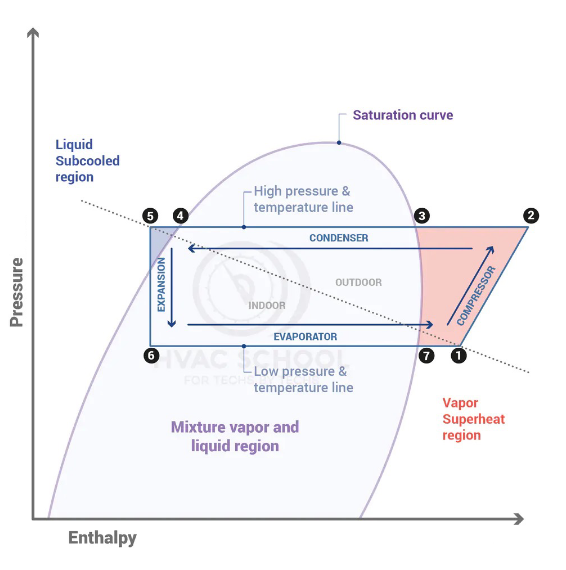
\includegraphics[width=0.6\linewidth]{IMAGES/LCA/Screenshot from 2024-11-04 11-32-23.png}
\end{figure}

\quad \underline{Coefficient of performance :}\\
\begin{itemize}
    \item $COP_{heating} = \frac{Q^-}{W^+}$
    \item $COP_{cooling} = \frac{Q^+}{W^-}$
\end{itemize}
COP are always greater than 1 as it does not take into account the energy from the ground.\\

We can also compute the carnot COP (ideal case): $COP_{carnot} = \frac{Q^-}{W^+_{min}} = \frac{T_h}{T_h-T_c}$, the carnot efficiency is then : $\varepsilon = \frac{COP}{COP_{carnot}}$.\\

\warning The ground average temperature is taken as $7^\circ C$.\\

\subsubsection{Sizing}
\begin{enumerate}
    \item Estimate the heat needs of the house (kWh per year) based on the current consumption of oil or gas
    \item Estimate the electricity needs of the heat pump (assuming a COP of 3) in kWh per year
    \item As heating is necessary only during a certain period, determine the size of the heat pump in kW
\end{enumerate}

\quad \underline{Types of heat pumps :}\\
Depends on where they take and release heat : \begin{itemize}
    \item Air-based : usually noisy, poorly efficient in winter. 
    \item Water-based : less noisy but require an open source of water. More efficient than air-based as the temperature of water is more constant.
    \item Ground-based : closed circuit of water (50 to 200m of depth). Most efficient type but expensive.
\end{itemize}

Heat pumps can operate up to $100^\circ C$ for heat production. New heat pumps reach up to $160^\circ C$. It can replace fossil sources for house heating, production of hot water but not for industrial heating.\\

\quad \underline{Refrigerant selection :}\\
\begin{itemize}
    \item Thermo-physical properties : temperatures and conditions, heat pump sizing, system performance
    \item Economics and environmental : system and refrigerant costs, measure of the impact related to $CO_2$, flammability
\end{itemize}

\subsection{Geothermal energy}
It is heat from the original formation of the planet and from radioactive decay.\\
Reserves and resources : \begin{itemize}
    \item hydrothermal : high temperature (water/steam at 100-400${}^\circ$C). Naturally occurring with the high temperatures of the rocks.
    \item Hot dry rock : geological formations abnormally hot but without water. Not naturally occurring water flows
    \item Deep aquifers : widely available. Reservoirs within the Earth with hot fluids.
\end{itemize}

Types of geothermal power plants : \begin{itemize}
    \item Dry-steam plants : only vapor ($27\%$ of worldwide capacity), direct use of geothermal steam
    \item Flash steam power plants (mixture of steam and liquid water, most common type $60\%$ of installed capacity)
    \item Binary cycle : similar to Rankine cycles
\end{itemize}

\subsection{Solar energy}
The irradiance at Earth's surface is : $I = \int_0^\infty E(\lambda, 5780K) d\lambda = 1000 W/m^2$.\\
The Global Horizontal Irradiance (GHI) or total radiation measured on a horizontal surface can be described as : $GHI = DHI + DNI \cos(\theta_s) W/m^2$ where $DHI$ is the Direct normal/beam radiation and $DNI$ the Diffuse Horizontal Radiation.\\
The total radiation on an inclined surface is then : $g_i = d_i+b_i$ with the beam component $b_i = DNI \cos(i)$ and $d_i = d_h \cdot 0.5 \cdot (1+\cos(i))$ ($d_h = GHI-DHI\cos\theta_s$).\\
How to harvest solar energy : \begin{itemize}
    \item Photoconversion ($\eta = 20\%$, to electricity)
    \item Thermalisation ($\eta = 50\%$, to heat)
    \item Thermochemical reaction ($\eta = 12\%$, to fuel)
\end{itemize}

\begin{equation}
    I = 1.1 I_0 0.7^{AM^{0.678}}
\end{equation}


\subsubsection{Solar to Electricity}

efficiency : $\eta = \frac{E_{peak}}{I_r S_{cell}}$\\
Increase voltage by connecting cells in series. The industrial standard is 60 or 72 cells in series.\\
\begin{enumerate}
    \item A photon hits an electron-hole pair
    \item The electron and the hole split and move around
    \item The electron gets dragged by the electric field of the P-N junction
    \item The electron and the hole are collected at the contacts
\end{enumerate}
Photons with energy greater than the band gap energy are absorbed to create free electrons and holes. Photons with less energy pass through the material without PV effect.\\
A solar cell in its own is very thin (250um) and very brittle. To protect it, ensure long term usage they are encapsulated in modules.\\
In first approximation, a PV behaves as a diode. It shows a high potential with no current or high current with no potential.\\
The Fill Factor is defined as : $FF = \frac{P_{MPP}}{I_{sc} V_{oc}}$. \\

The Energy Payback Time (EPBT in years) is expressed as : $EPBT = \frac{E_{in}}{E_{out}}$.\\

Different concepts : \begin{itemize}
    \item Self consumption : you consume part of what you produce
    \item Self sufficiency : you produce part of what you consume
    \item Autonomy : you produce all you need, without need of the grid to buy or sell
    \item Neutrality : over a year, you've produced what you've consumed
\end{itemize}

\subsubsection{Solar to heat}
Two main approaches : \begin{itemize}
    \item Non or low concentrating : ($30^\circ C < T < 240^\circ C$), working fluid (air, water, oil)
    \item Concentrating : high to very high temperature range ($300^\circ C < T < 1000^\circ C$), working fluid (water, molten salt)
\end{itemize}

Mostly used for electricity generation. Advantages : higher temperature/efficiencies achievable; reflecting surfaces requires less material. Disadvantages : no diffuse radiation collected; may require tracking: reflecting surfaces degrades with time.\\

\subsubsection{Solar to fuel}

In general, it is the cracking of elements such as $H_2O$ to generate Hydrogen.\\

\subsection{Wind energy}
Wind can be defined as : \begin{itemize}
    \item Differences in pressure caused by uneven solar heating on the earth surface
    \item Rotation of the Earth : Coriolis force
    \item Friction close to the Earth surface
\end{itemize}
The power of wind in a given area : $\dot{E}_{k,air} = \frac{1}{2}\rho A v_0^3$ and the force (drag) is then : $F_{air} = \frac{1}{2}\rho A v_0^2$.\\
World wind capacity installed : 1021GW. Wind production 2311 TWh/y (capacity factor of $25\%$, $7.8\%$ of world electricity supply).\\
Onshore windmills represent $72\%$ of new installations.\\
The wind speed distribution at a given site is given by the Weibull probability density function : $f(v) = (\frac{k}{c}) (\frac{v}{c})^{k-1} e^{-(\frac{v}{c})^k}$.\\

Let's consider a control volume V. $P_{in}-P_{out} = \frac{1}{2} \rho (v_0^2-v_2^2)$.\\
The kinetic energy is then : $\dot{E}_T = C_p \dot{E}_{wind}$ with $C_p = \frac{A_2}{A_T} \frac{v_2}{v_0} (1-(\frac{v_2}{v_0})^2) = \frac{(1+x)(1-x^2)}{2} K$ with $x =\frac{v_2}{v_0}$.\\

\warning Betz law gives us a theoretical limit for the efficiency; we can harvest at most $59.3\%$ of the energy of the wind. (In real world application we are between $35-50\%$)\\

Losses : \begin{enumerate}
    \item Wake loss 
    \item Top losses : blade tips thermselves also create vortices
    \item Drag losses : blades rotating through air experience a resistance
\end{enumerate}

\quad \underline{Types of :}\\

\begin{itemize}
    \item Vertical axis. Can be drag (Savonius rotor) or lift based (Darrieus rotor).
    \item Horizontal axis. Most used and efficient.
\end{itemize}

Key parameters :\begin{itemize}
    \item Number of blades : does not influence the power. 
    \item Rated power
    \item Hub height
    \item Swept area
    \item Solidity (blade area/swept area) : high leads to high starting torque and low speed
\end{itemize}


\quad \underline{Wind farms :}\\

Wind turbines are used in wind farms : \begin{itemize}
    \item Usually 10-30 turbines
    \item Spacing 7-8 diameters
    \item 1 grid transformer for the whole site 
    \item Timing : construction (1y), operation (20y), decommissioning (0.5y)
\end{itemize}

Capacity factor ($c_f = \frac{\int_{year} \dot{E}(t) dt}{\dot{E}_{rated} \cdot 8760}$) : \begin{itemize}
    \item Onshore : $c_f = 25\%$
    \item Offshore : $c_f = 35\%$
\end{itemize}

And the Levelised Cost of Electricity is about $35-80 $€/MWh onshore and $70-120$€/MWh offshore.\\

\quad \underline{Risks and impacts :}\\

\begin{itemize}
    \item Machinery maintenance accidents
    \item Blade failures
    \item Falling ice
    \item Paraglider and small aircraft crashing into support structures
    \item Turbine's brake fails 
    \item Turbine blades may fall
    \item Lightning strikes
\end{itemize}


\subsection{Hydropower}
Three types of hydro power plants : \begin{itemize}
    \item Run-of-river
    \item Hydro dam (storage)
    \item Pumped storage
\end{itemize}

In Europe, hydro corresponds to $15\%$ of the electricity production. (In Switzerland, it is close to $60\%$).\\
We have : $gH_1 - gH_2 = g(z_U-z_L) - \sum gH_r$ with $gH_r$ the losses. The degree of reaction of then $\tau_r = \frac{e_p}{e_{12}}$ with $e_p = (gz_1 + \frac{P_1}{\rho}) - (gz_2 + \frac{P_2}{\rho})$ the potential energy and $e_{12} = e_p + \frac{1}{2} (v_1^2 - v_2^2) - e_{loss}$. \\
The specific speed is then : $\nu = \frac{\omega Q^{1/2}}{\pi^{1/2} (2e)^{1/4}}$.\\

\begin{itemize}
    \item Pelton : Efficiency up to $92\%$. Power up to $400MW_e$. High head, low discharge.
    \item Francis : most used and versatile type ($\simeq 60\%$ of installed capacity). Reaction turbine. Medium head. Wheel diameters ($0.5-8m$). Efficiency between $96-97\%$.
    \item Kaplan/bulb : Low head. Run-of-river plants. High discharge. Typical power : $5-200MW_e$.
\end{itemize}

Efficiency of a turbine : \begin{equation}
    \dot{E} = \dot{m} \omega_{12} \eta_T \eta_{gen} \eta_{gear} \eta_{transfo}
\end{equation}
With : \begin{itemize}
    \item $\eta_T = 92\%$ : mechanical efficiency
    \item $\eta_{gear} = 98\%$ : efficiency of the gear box
    \item $\eta_{gen} = 97\%$ : efficiency of the generator
    \item $\eta_{transfo} =98\%$ : efficiency of the transformer
\end{itemize}

For a capacity factor of $50\%$, the LCOE is about $28-90 USD/MWh_e$.\\

With pumped-hydro storage, the round-trip efficiency is about $80\%$.\\

\subsection{Biomass}
Biomass is all living matter on Earth. Depending on the time frame, it can be admitted as renewable energy. Photosynthesis is the conversion of light into stored chemical energy. It is described by the Calvin cycle : $n CO_2 + nH_2O + \text{sunlight} \rightarrow C(H_2O)_n + n O_2$.\\
The biomass is composed of : \begin{itemize}
    \item Dry matter : organic matter(Cellulose + Hemicellulose + Lignin + Extractives) + ash
    \item Moisture
\end{itemize}
The organic matter is composed of $50\%C$(wt) and $40\%O$(wt).
\begin{itemize}
    \item Dry biomass : lignocellulosic most abundant,wood and co-products, agricultural co-products, energy crops
    \item Wet biomass : more than $50\%$ moisture, agricultural products, industry co-products, organic waste
    \item Marine biomass : extracted/produced from ocean sources, algae
\end{itemize}

The vegetation stores about $2300 GtC$ while the atmosphere stores $600GtC$. The carbon-neutral aspect : \begin{itemize}
    \item direct $CO_2$ emissions : combustion of biomass
    \item indirect $CO_2$ emissions : land use change, forest management, harvesting/transportation
\end{itemize}

Biomass contains about $33$ to $60\%$ less energy than fossil fuels (weight basis) because of the presence of O in the molecule.\\
\warning The lower heating value of biomass is : $15-20MJkg$ on a dry basis.\\
In the world, about $66\%$ of the biomass is used for cooking and heating. \\

The use of biomass for bioenergy competes with food supply. \\
Conversion : \begin{itemize}
    \item Combustion : $\eta = 35\%$, generation of PM, CO, PAH, NO/$NO_2$, $SO_2$, HCl, $\cdots$
    \item gasification : generation of biofuel. Needs heat to generate gas. Production of synthetic natural gas : dry the wood, gasify it, gas clean-up, methane synthesis and then $CO_2$ removal. Up to $70\%$ of the energy input is transferred into the methane.
    \item Power to gas concept : long term electricity storage by converting electricity to fuel. $\eta_c = 85\%$. During winter, one can transform wood into SNG, useful het, waste heat and net electricity whereas during summer, one can transform wood + $H_2$ into SNG useful heat and waste heat in larger quantity.
    \item Liquid fuel synthesis : biomass to syngas. Syngas by indirect fluidized bed gasification, cold gas cleaning. 
    \item Pyrolisis : temperature zone above drying but below gasification. 
    \item Biomethanation : ($50\%$ of energy transferred to produce biogas) put biomass in a reservoir and wait for the bacteria to produce methane. Process is slow (weeks) and don't need high temperature (ambient).
    \item Fermentation : extract sugar from biomass and let it sit to produce ethanol ($26.8 MJ/kg$)
\end{itemize}

\subsection{Storage}
There are three kinds of efficiency : Charging efficiency $\eta_{charge}$, discharging efficiency $\eta_{discharge}$, round-trip efficiency $\eta_{charge} \times \eta_{discharge}$. Storage consumes electricity ($0.3\%$ of all electricity generated in the US). Self-discharge losses. Power density is defined as how fast energy can be stored and discharged, expressed in W/kg. Energy density is defined as how much energy can be stored, in J/$m^3$ or in J/kg.\\

Classification :
\begin{itemize}
    \item Mechanical : pumped hydro energy storage (widespread technology, round-trip efficiency between $70-85\%$, low energy density $0.5-5 kWh/m^3$ or $200-2000m^3$ of water to store $1MWh$, low power density), compressed air energy storage (air compression and fuel combustion to increase the turbine inlet temperature, $W_{max} = p_2 V_2 \ln(p_2/p_1) + (p_2-p_1)V_2$, well-known technology, round-trip efficiency of $27-70\%$, geographical limitations, $200m^3$ of air to store $1MWh$)
    \item Thermal : latent ($Q = m \Delta h_{phase\: change}$, phase-changing materials, round-trip efficiency of $80-90\%$, versatile, higher energy density than sensible, efficiency depends on material, can be expensive), sensible ($Q = mc_p \Delta T$, we increase/decrease its temperature, round-trip efficiency of $80-90\%$, inexpensive, safe, limited energy density)
    \item Electrical : super capacitors
    \item Electrochemical : batteries (chemical reactions to enable the flow of electrons, cathode gets reduces and anode gets oxidized, well suited for small and large scale applications, round-trip efficiency of $75-90\%$, low energy density i.e. $150Wh/kg$ for lithium-ion, self-discharge issues)
    \item Chemical : Power-2-X (chemical reactions driver by electricity to generate a chemical fuel, first water electrolysis, then methanation, then injection and transport, finally use, round-trip efficiency between $30-50\%$, low efficiency, hydrogen storage, investment cost)
\end{itemize}

\subsection{Fuel cells}
$H_2$ has uses in all sectors. It is coupled to rise in wind and PV power. A fuel cells works like a gas battery. Chemical fuel is directly converted into electricity and useful heat. Gases are consumed and electrodes are invariable. Increase electrode surface means high current I. The 2 fuel cell types (Phosphoric Acid Fuel Cell PAFC $40\%$eff., Polymer Membrane FC PEM/PEFC $50\%$eff.) use proton conduction in a liquid or a wet membrane. They operate at $200^\circ C$ (acid) or below $100^\circ C$. At this temperature, the only fuel reactive enough to be oxidized is hydrogen. The only electrodes capable to catalyze this reactive in acidic medium at such low temperature are the noble metals. \\
Then, we also have Alcaline Fuel cell for mobility (temperature of $80^\circ C$); Solid Oxide Fuel cell for cogeneration ($60\%$eff., temperature of $600-1000^\circ C$); Molten Carbonate Fuel cell for cogeneration ($50\%$eff., temperature of $600^\circ C$).\\

Physico-chemical processes occur in/on the electrodes and at the electrode/electrolyte interfaces. These cause voltage losses which are non-linear with current. The efficiency of the cell is then : $\eta_{cell} = \eta_I \eta_V \eta_{THDYN}$, with $\eta_I = \frac{I}{fnF}$ the current efficiency, $\eta_{V} = \frac{E_{cell}}{E_{nernst}}$ the voltage efficiency and $\eta_{THDYN} = \frac{\Delta G(p,T)}{\Delta H_{293K}}$ the thermodynamic efficiency. Part-load efficiency is greater than full load efficiency. \\
Any hydrocarbon fuel is converted to syngas ($H_2$, $CO$). Syngas can directly feed high temperature FC. To feed low temperature FC, chemical steps are needed to reduce CO content to traces as CO blocks the Pt-catalyst. \\






\end{document}